%!TEX root = ../Technische Dynamik.tex

\tikzstyle{hatch}=[postaction={draw,decorate,decoration={border,angle=-45, amplitude=0.15cm,segment length=1.2mm}}]

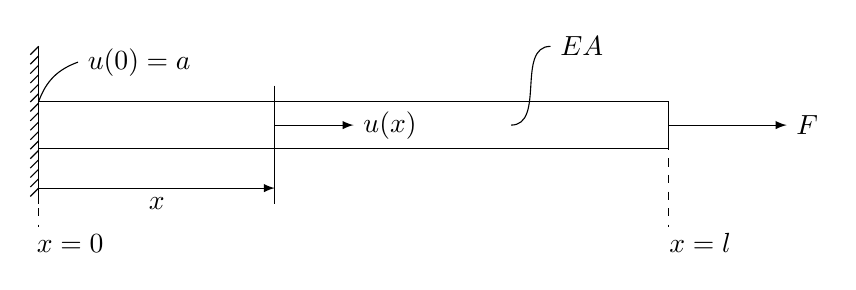
\begin{tikzpicture}[>=latex]

\draw[hatch] (0,1) -- (0,-1);
\draw (0,-0.3) rectangle (8,0.3);
\draw (3,0.5) -- (3,-1);
\draw[->] (0,-0.8) -- node[below] {$x$} (3,-0.8);
\draw[dashed] (0,0) -- (0,-1.3);
\draw[dashed] (8,0) -- (8,-1.3);
\node at (0.4,-1.5) {$x=0$};
\node at (8.4,-1.5) {$x=l$};

\draw[->] (3,0) -- (4,0) node[right] {$u(x)$};
\draw[->] (8,0) -- (9.5,0) node[right] {$F$};

\draw (0,0.3) to[out=70,in=200] (0.5,0.8) node[right] {$u(0)=a$};
\draw (6,0) to[out=0,in=180] (6.5,1) node[right] {$EA$};

\end{tikzpicture}